\section{The sample}
\label{sec:sample}

This search covers \NWindows{} spectral windows toward \NStars{} stars in
\NSystems{} systems within 40\,pc. They come from \NEB{} public ALMA execution
blocks put through one pipeline: \TotalDataTB\,TB of raw data, \StTelHours\,h
of telescope time and \LdgCensusHours\,h summed over windows. This
\emph{primary census} is the set over which every sensitivity, expectation and
limit is computed. It holds \CsNCross{} of the \EvNCrossRaw{} threshold
crossings this paper reports, all in quality-passing data. The remaining \CeNTailCross{}
lie in an \emph{archival tail} of \LdgExtTail{} blocks toward
\LdgTailStars{} census stars, searched after the census was closed, and enter
no expectation. Nor do an archival extension, a reserved \emph{hold-out}
(Appendix~\ref{sec:heldout}) and a control beyond 40\,pc
(\S\ref{sec:holdoutsearch}). Table~\ref{tab:blockledger} accounts for every
set, and Table~\ref{tab:counts} gives the set each count is taken over. A
\emph{system} is a bound group, counted once however many of its stars were
observed.

The census is two experiments, divided on native channel width, on which both
the search statistic and the completeness calibration depend.
\emph{Class~A}, the primary experiment, is the \NWinA{} fine-channel windows
toward \LdgClassAStars{} stars in \NSysClassA{} systems. Of these, \EtaDriftAOk{}
are channelised finely enough for the searched drift to cross a channel
(\S\ref{sec:statistic}), and every sensitivity and limit quoted is Class~A's
unless stated otherwise. \emph{Class~B}, the other \NWinB{} windows, supports a
secondary search for an unresolved spectral excess. The channelisation is
bimodal, so the division is unambiguous: the widest fine channel is
\ScChanFineMaxMHz\,MHz and the narrowest coarse one \ScChanCoarseMinMHz\,MHz,
with nothing between them.

A star enters if its Gaia~DR3 parallax is at least 25\,mas and measured to
better than \PlxAdqlPct{} per cent, a clause that never binds (the worst among
the stars searched is \SfPlxWorstPct{} per cent). Its proper-motion-corrected
position must fall inside the quoted field of view of a public execution
block, though not necessarily at the pointing centre, and its distance is
$1/\varpi$. A window is kept only where the primary-beam response at the star
is at least \BmFloorResp, where the adopted Gaussian and a blocked-aperture
response part by \BmFloorTolPct{} per cent; no window falls below it
(Appendix~\ref{app:pbresp}). Of the \NCensus{} work-list entries the query
returns, only \NGenuinelyCovered{} stars prove to lie inside a public field,
and \NStars{} yielded a searchable window. One serendipitous field star is
named throughout after the ALMA source at its field centre, \BkAlmaName: it is
\BkAlmaTwoMass{} (Gaia~DR3 \BkAlmaGaia), an \BkAlmaSpType{} dwarf at \BkAlmaDistPc\,pc with no
catalogued radial velocity.

A star with no Gaia~DR3 parallax cannot enter. That removes all \BsNBright{}
stars in this volume brighter than \BsBrightMag{} magnitude, and \BsNGap{} of
its \BsNVol{} qualifying Hipparcos stars in all, \BsGapNFaint{} of them
fainter than Hp~\BsGapMagCut. Of these, \BsNAlmaWord{} lie in public fields:
\BsStarList, with \BsNWinA{} fine-channel and \BsNWinB{} coarse-channel windows
(\BsRawTB\,TB in \BsNEB{} blocks) that a search admitting Hipparcos astrometry
could add.


\subsection{The archival selection}
\label{sec:bias}

This sample was not designed: it is whatever ALMA programmes with other aims
happened to observe among the stars Gaia~DR3 catalogues, and \PctDiscProposal{} per cent
of the stars searched were targeted under a debris-disc or planet-formation
proposal. Table~\ref{tab:selfunc} measures the bias against the volume-limited
Gaia~DR3 census of which the searched stars are a subset ($\varpi>0$,
$\sigma_\varpi/\varpi\le\SfPlxCutDec$, $1/\varpi\le40$\,pc; \SfCensusN{}
objects). Both columns are classified by BP$-$RP colour, with absolute $G$
magnitude separating the degenerates.

Distance is the dominant selection effect: stars within 5\,pc are
over-represented by a factor \SfTopRatio, falling monotonically to a factor of
two \emph{under}-representation beyond 30\,pc. Colour comes second. A~stars are
over-represented by about \SfARatio{} and F and G stars by factors of three,
because those are the stars with bright debris discs. For the A~stars that
factor is a floor, since the Gaia requirement itself removes stars that blue
at \BsEarlyRatio{} times its rate among the others. M~dwarfs are depleted:
\SfMSearched{} of the \SfNStar{} searched stars, a factor \SfMRatio{} of their
share of the census, and only \SfMClassAStars{} of them carry fine-channel
coverage. Coverage is concentrated too, \ConcThreeWin{} of the \NWindows{}
windows coming from \ConcThreeSys{} systems. The selection acts hardest on the
targets a designed search would pick: of the \CsIntNRow{} sample systems within
15\,pc with a confirmed planet, \CsIntNoClassA{} have no Class~A coverage and so
no drift-resolving limit. No statement in this paper is therefore an
occurrence rate for the solar neighbourhood.

%% GENERATED by selfunc_v411.py -- do not hand-edit.
\begin{table}
\centering
\scriptsize
\setlength{\tabcolsep}{4pt}
\caption{Selection function of the 90 searched stars against the volume-limited Gaia~DR3 census of \S\ref{sec:bias}. ``Ratio'': the searched over the census column fraction.}
\label{tab:selfunc}
\begin{tabular}{@{}lrrr@{}}
\toprule
Property & Census & Searched & Ratio \\
\midrule
\multicolumn{4}{@{}l}{Distance} \\
\quad $d\le5$\,pc & 48 (0.3\%) & 13 (14.4\%) & 52.9 \\
\quad 5--10\,pc & 240 (1.4\%) & 13 (14.4\%) & 10.6 \\
\quad 10--20\,pc & 2069 (11.8\%) & 18 (20.0\%) & 1.7 \\
\quad 20--30\,pc & 5391 (30.7\%) & 19 (21.1\%) & 0.7 \\
\quad 30--40\,pc & 9818 (55.9\%) & 27 (30.0\%) & 0.5 \\
\midrule
\multicolumn{4}{@{}l}{Colour class$^{a}$} \\
\quad A & 61 (0.4\%) & 5 (6.2\%) & 17.2 \\
\quad F & 473 (2.8\%) & 8 (10.0\%) & 3.6 \\
\quad G & 978 (5.8\%) & 15 (18.8\%) & 3.2 \\
\quad K & 2221 (13.2\%) & 11 (13.8\%) & 1.0 \\
\quad M & 13\,082 (77.8\%) & 41 (51.2\%) & 0.7 \\
\midrule
\multicolumn{4}{@{}l}{Other axes} \\
\quad Confirmed planet hosts$^{b}$ & 26 (15.5\%) & 24 (26.7\%) & 1.7 \\
\quad White dwarfs$^{a}$ & 463 (2.7\%) & 8 (9.1\%) & 3.4 \\
\quad Searched stars / systems & -- & 90 / 83 & -- \\
\bottomrule
\end{tabular}

\smallskip
{\footnotesize $^{a}$Colour bins, not MK types: BP$-$RP $<0.36$ for A, 0.36--0.72 for F, 0.72--0.95 for G, 0.95--1.77 for K and $>1.77$ for M, where the census's own temperature--colour relation crosses 7500, 6000, 5300 and 3900\,K. Degenerate: more than 4\,mag below the census main sequence. The five classes are normalised over the 80 non-degenerate searched stars and the 16\,815 non-degenerate census objects, the degenerate row over the 88 classified searched stars and the 17\,278 classified census objects.\\ $^{b}$Both columns are the same positional join, of the 168-entry ALMA-covered work list and of its searched subset, to the NASA Exoplanet Archive \texttt{pscomppars} table accessed 2026 October 4. The 24 searched hosts carry 51 confirmed planets, 22 of the 24 surviving the deuterium-burning mass limit; the Gaia census carries no planet information, so the census column in this row is the work list and not the 17\,566-object Gaia census.}
\end{table}


\subsection{Frequency coverage and archival scope}
\label{sec:coverage}

The Class~A experiment covers $\Delta\nu_A=\DnuA$\,GHz of unique sky
frequency, in \DomAIslands{} disjoint islands between \DomAFreqLo{} and
\DomAFreqHi\,GHz rather than a band. With the coarse-channel windows the
coverage is \DnuAB\,GHz in \UnionIntervals{} intervals, of which
\SearchedUnionGHz\,GHz survives the molecular-line mask of
\S\ref{sec:summary}. Fig.~\ref{fig:waterfall} shows the distribution: a
transmitter between the islands was never observable here, whatever its
power. Nor is the archive exhausted: \LdgExtScope{} further blocks inside the
same query were unprocessed when the census was frozen, \FateNoCal{} of them
(\FateNoCalGB\,GB) because the archive holds their raw visibilities but never
pipeline-calibrated them (Table~\ref{tab:blockledger}).

\begin{figure*}
\centering
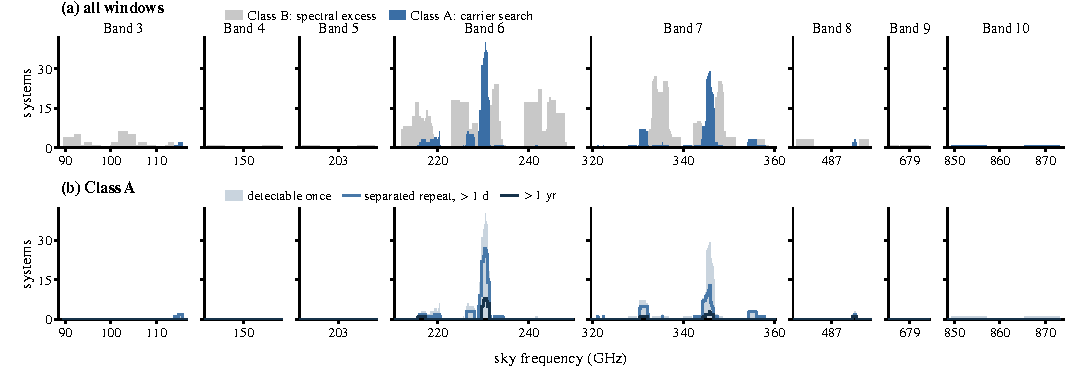
\includegraphics[width=\textwidth]{figures/coverage_r27.pdf}
\caption{\textbf{Where this survey searched, and where a repeat could test
it}: independent systems covering each sky frequency, one panel per populated
ALMA band, its width proportional to the band's frequency share; curves step
at the searched window edges. \emph{(a)}~Every window: blue, the
fine-channel carrier search (Class~A); grey, the coarse-channel
spectral-excess search (Class~B); the summed window bandwidth is
$\GrossOverUnion\times$ the union. \emph{(b)}~Class~A: detectable once (grey);
with a \emph{separated} block (Table~\ref{tab:quantities}) covering the
frequency (blue); beyond a year (dark). An accelerating carrier further needs
a matching orbital phase.}
\label{fig:waterfall}
\end{figure*}
